% Software Overview
% MIT License
%
% Copyright (c) 2026 HumberASV
% Copyright (c) 2026 Carson Fujita
%
% Permission is hereby granted, free of charge, to any person obtaining a copy
% of this software and associated documentation files (the "Software"), to deal
% in the Software without restriction, including without limitation the rights
% to use, copy, modify, merge, publish, distribute, sublicense, and/or sell
% copies of the Software, and to permit persons to whom the Software is
% furnished to do so, subject to the following conditions:
%
% The above copyright notice and this permission notice shall be included in all
% copies or substantial portions of the Software.
%
% THE SOFTWARE IS PROVIDED "AS IS", WITHOUT WARRANTY OF ANY KIND, EXPRESS OR
% IMPLIED, INCLUDING BUT NOT LIMITED TO THE WARRANTIES OF MERCHANTABILITY,
% FITNESS FOR A PARTICULAR PURPOSE AND NONINFRINGEMENT. IN NO EVENT SHALL THE
% AUTHORS OR COPYRIGHT HOLDERS BE LIABLE FOR ANY CLAIM, DAMAGES OR OTHER
% LIABILITY, WHETHER IN AN ACTION OF CONTRACT, TORT OR OTHERWISE, ARISING FROM,
% OUT OF OR IN CONNECTION WITH THE SOFTWARE OR THE USE OR OTHER DEALINGS IN THE
% SOFTWARE.

% Specifications for the basestation and web client application
\subsection{Base Station Specifications}
\label{sec:basestation-specifications}
The basestation is responsible for receiving data from the ASV for diagnostic monitoring and hosting the web client.

It will host the following endpoints:

\begin{description}
    \label{itm:endpoints}
    \item[\textit{/admin}] The admin webpage that allows technical users to manage secure tokens for user access, including creating, revoking, and expiring tokens as needed to maintain security.
    \item[\textit{/admin/create\_token}] An endpoint for the admin webpage to create secure tokens for user access.
    \item[\textit{/admin/revoke\_token}] An endpoint for the admin webpage to revoke secure tokens for user access.
    \item[\textit{/admin/expire\_token}] An endpoint for the admin webpage to expire secure tokens for user access.
    \item[\textit{/admin/tokens}] An endpoint for the admin webpage to get a list of all active tokens for user access.

    \item[\textit{/client}] The web client application to access the streaming data with a valid token.
    \item[\textit{/uh\_oh}] An endpoint to handle unauthorized access attempts and display an appropriate error message to users who do not have valid tokens or permissions to access the application.
\end{description}

\subsubsection{Operating Environment}
The Base Station software will be designed to run on a Windows, Linux, or macOS computer that can connect to the ASV's access point. 
The web client application will be accessible through a web browser and will not require any additional software installation for user access. The system will need to be compatible with common web browsers such as Google Chrome, Mozilla Firefox, and Microsoft Edge to ensure accessibility for all users. The Base Station software will need to be able to run on a variety of hardware configurations, as the team may use different computers for development and testing. The system will also need to be designed to operate in environments with limited connectivity and potential interference, such as during maritime competitions where there may be multiple teams and devices operating in close proximity.
Loon-E runs on a Jetson Orin with Ubuntu Jammy Jellyfish (22.04) and uses ROS Humble and Jetpack 5.0. A corresponding ROS node must be implemented to transmit data from the ASV to the Base Station. The Base Station and web client are isolated from the ROS enviroment and do not require compatibility considerations with it.

\subsubsection{Functional Requirements}
\begin{itemize}
    \item FR-23: The Base Station application shall connect to the ASV using Cyclone DDS communication protocols.
    \item FR-24: The Base Station application shall relay the received data through TCP from the ASV to the web client application for visualization and monitoring by users.
    \item FR-25: The Base Station application shall handle the authentication and security of the connection with salt-based hashing and token management to ensure that only authorized users can access the data.
    \item FR-26: The Base Station application shall host a website for the web client application.
    \item FR-27: The Base Station application endpoints shall reject unauthorized access attempts and display an appropriate error message to users who do not have valid tokens or permissions to access the application.
    \item FR-28: The Base Station shall use the endpoint \textit{/admin} for the admin webpage that allows technical users to create, revoke, or expire tokens as needed to maintain security.
    \item FR-29: The Base Station shall use the endpoint \textit{/admin/create\_token} for the admin webpage to create secure tokens for user access.
    \item FR-30: The Base Station shall use the endpoint \textit{/admin/revoke\_token} for the admin webpage to revoke secure tokens for user access.
    \item FR-31: The Base Station shall use the endpoint \textit{/admin/expire\_token} for the admin webpage to expire secure tokens for user access.
    \item FR-32: The Base Station shall use the endpoint \textit{/admin/tokens} for the admin webpage to get a list of all active tokens for user access.
    \item FR-33: The Base Station shall use the endpoint \textit{/client} for the web client application to access the streaming data with a valid token.
    \item FR-34: The Base Station shall use the endpoint \textit{/uh\_oh} to handle unauthorized access attempts and display an appropriate error message to users who do not have valid tokens or permissions to access the application.
    \item FR-35: The Base Station shall allow technical users to create a admin user account through terminal commands.
    \item FR-36: The Base Station application shall allow the admin user to create, revoke, or expire tokens as needed to maintain security.
\end{itemize}


% Specifications for web client application
\subsection{GUI Development}

Following \hyperref[sec:basestation-previous-implementation]{the previous implementation of the base station}, we have decided to implement with Flask instead of Django for the web server component of the base station.
Flask is a lightweight web framework\autocite{FLASK} which can also scale and handle the \hyperref[sec:basestation-user-needs]{user needs} of our web client application without the overhead of Django's features that we do not require.

We will use flask to create a web server that will handle the following tasks:

\begin{itemize}
    \item create an API for handling security tokens (under \hyperref[itm:fr-webclient-token]{FR-21} and \hyperref[itm:fr-webclient-admin]{FR-22}) 
    \item to serve the web client application to users.
    \item stream the video feed from process 2.8 (Telemetry) in Figure \ref{fig:base-station-diagram} to the web client application.
    \item stream telemetry data from process 2.8 (Telemetry) in Figure \ref{fig:base-station-diagram} to the web client application for visualization.
\end{itemize}

\subsubsection{Streaming Video and Telemetry Data}

\subsubsection{Security Token Management}
Before serving the \textit{/client} page, the website host verifies that telemetry and video streams from the ASV are being received. 
If the streams are unavailable, the site displays an error page and access to the web client is withheld until data reception resumes. 
When streams are available, the host prompts the user to enter a token (see the ``Get Login page'' step in the sequence diagram, Figure \ref{fig:seq-connection}). 
The submitted token is sanitized and checked against the database (D1 in Figure \ref{fig:base-station-diagram} and Figure \ref{fig:seq-connection}); 
a valid token grants access to the web client and its live telemetry and video, while an invalid token results in an error page denying access. 
This behavior implements the token API (\hyperref[itm:fr-webclient-token]{FR-21}) and the admin token management features (\hyperref[itm:fr-webclient-admin]{FR-22}), 
ensuring only authorized users may view ASV data and video feeds.

\begin{figure}[H]
    \centering
    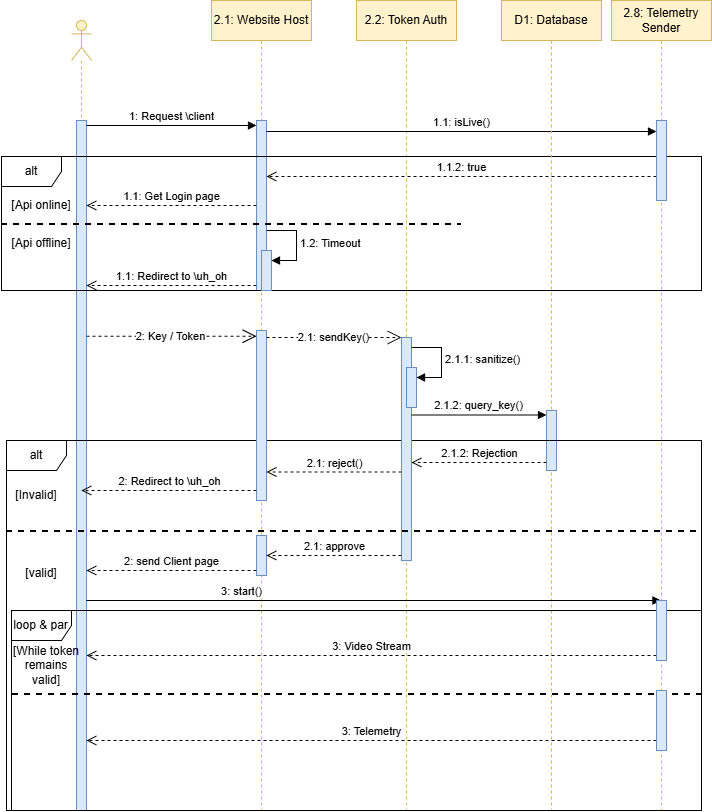
\includegraphics[width=0.8\textwidth]{./images/GUI/sequence-connection.png}
    \caption{Sequence Diagram for User Connection to Web Client}
    \label{fig:seq-connection}
\end{figure}

\notebox{Technical users, such as the Humber ASV team, will have access to an admin webpage within the web client application that allows them to create, revoke, and expire tokens as needed to maintain security.}


\subsubsection{Functional Requirements}
\begin{itemize}
    \item FR-1: The web client application shall display the ASV's speed over ground in meters per second.
    \item FR-2: The web client application shall display the ASV's heading.
    \item FR-3: The web client application shall display the ASV's current task status.
    \item FR-4: The web client application shall display the ASV's battery levels.
    \item FR-5: The web client application shall display the ASV's task data.
    \item FR-6: The web client application shall display a map showing the ASV's position and route.
    \item FR-7: The web client application shall display the signal strength of the connection between the ASV and the Base Station.
    \item FR-8: The web client application shall display a log from the ASV that includes relevant information about the ASV's operations and status.
    \item FR-9: The web client application shall display a power and rudder panel that shows the power allocation in the propeller and the rudder angle.
    \item FR-10: The web client application shall display received image recognition data from the ASV, such as object detection windows from the Zedx camera.
    \item FR-11: The web client application shall display image recognition data as boxes overlaid on the video feed from the Zedx camera.
    \item FR-12: The web client application shall be accessible through the latest (as of 2026) common web browsers and shall not require any additional software installation for user access.
    \item FR-13: The web client application shall have a border color that indicates the ASV's status, such as autonomous, remote control, standby, out of control, or lost connection.
    \item FR-14: The web client application shall use green border color to indicate autonomous mode.
    \item FR-15: The web client application shall use blue border color to indicate remote control mode.
    \item FR-16: The web client application shall use yellow border color to indicate standby mode.
    \item FR-17: The web client application shall use red border color to indicate out of control status.
    \item FR-18: The web client application shall use gray border color to indicate lost connection status.
    \item FR-19: The web client application shall update the border color in real-time based on the ASV's status.
    \item FR-20: The web client application shall have webpage with a text field that requires a valid token.
    \item FR-21: The web client application shall require a valid token to access and view the streaming data.
    \label{itm:fr-webclient-token}
    \item FR-22: The web client application shall have an admin webpage that allows technical users to manage secure tokens for user access, including creating, revoking, and expiring tokens as needed to maintain security.
    \label{itm:fr-webclient-admin}
\end{itemize}

\subsubsection{ASV}
\begin{itemize}
    \item FR-37: The ASV shall collect data from various sensors and systems on the ASV, such as telemetry data, sensor readings, and video feeds from the Zedx camera.
    \item FR-38: The ASV shall transmit the collected data to the Base Station application using Cyclone DDS communication protocols.
\end{itemize}

\newpage % Start a new page for the next section